\documentclass[tikz,border=2pt]{standalone}

\usepackage[utf8]{inputenc}
\usepackage{pgf}
\usepackage{tikz}
\usetikzlibrary{arrows,automata}

\begin{document}

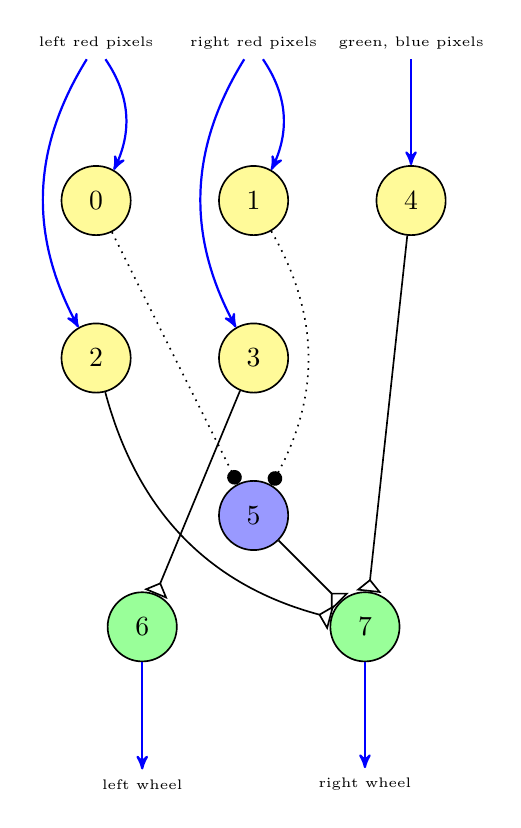
\begin{tikzpicture}[->,>=stealth',auto,semithick,node distance=2cm]

    \node (lrp) {\tiny{left red pixels}};
    \node (rrp) [right of=lrp] {\tiny{right red pixels}};
    \node (gbp) [right of=rrp] {\tiny{green, blue pixels}};

	\node[state,fill=yellow!40] (q0) [below of=lrp] {0};
	\node[state,fill=yellow!40] (q1) [below of=rrp] {1};
	\node[state,fill=yellow!40] (q2) [below of=q0] {2};
	\node[state,fill=yellow!40] (q3) [below of=q1] {3};
	\node[state,fill=yellow!40] (q4) [below of=gbp] {4};

	\node[state,fill=blue!40] (q5) [below of=q3] {5};

	\node[state,fill=green!40] (q6) [below left of=q5] {6};
    \node[state,fill=green!40] (q7) [below right of=q5] {7};

    \node (lw) [below of=q6] {\tiny{left wheel}};
    \node (rw) [below of=q7] {\tiny{right wheel}};
	
	\path (lrp) edge[thick,draw=blue,bend left]  (q0)
	            edge[thick,draw=blue,bend right] (q2)
	      (rrp) edge[thick,draw=blue,bend left]  (q1)
	            edge[thick,draw=blue,bend right] (q3)
	      (gbp) edge[thick,draw=blue] (q4)
	      (q0)  edge[dotted,-*] (q5)
	      (q1)  edge[dotted,bend left,-*] (q5)
	      (q2)  edge[bend right,-open triangle 90 reversed] (q7)
	      (q3)  edge[-open triangle 90 reversed] (q6)
	      (q4)  edge[-open triangle 90 reversed] (q7)
	      (q5)  edge[-open triangle 90 reversed] (q7)
	      (q6)  edge[thick,draw=blue] (lw)
	      (q7)  edge[thick,draw=blue] (rw);

\end{tikzpicture}

\end{document}
